\section{Experimental setup}\label{subsection:set-up}

The experimental setup is depectied in \cref{fig:setup}. The setup is driven by a modelocked Ti:sapphire laser. The laser emits femtosecond pulses at a wavelength of \qty{810}{\nm}, with a repetion rate of \qty{80}{\MHz} and an average output power of \qty{4}{\W}. The laser beam then passes through an optical parametric oscillator (OPO), where the beam undergoes nonlinear frequency conversion resulting in two waves: an idler wave and a signal wave. The OPO idler wave can be tuned from \qtyrange{1.7}{4}{\um} and has a maximum output power of \qty{650}{\mW}. The idler has been tuned to a specific wavelength of \qty{2071.7}{\nm} and was stabilzied using an integrated automated feedback loop.

To further achieve a wide range of pulse fluences, the laser beam is directed through two wire-grid polarizers. One of the polarizers is placed on a controllable rotation stage to adjust the beam attenuation. The wire-grid polarizers have a broad range of attenuation across different wavelengths and do not alter the beam path during rotation. After the attenuation stage, the beam passes through a beamsplitter, which separates it into two arms: the reference arm and the sample arm. 

The reference arm contains a high-reflection mirror, from which a portion of the beam is leaked and collected by a photodiode
The reference arm contains a high-reflection mirror from which the leaking signal is collect in a photo diode to monitor the fluence during a measuremnt. 
The sample in this experiment refers to a VECSEL chip and is placed at the end of the sample arm. Before the beam is incident on the sample, a focusing lens is used to achieve higher fluences on the VECSEL. The VECSEL is probed under a direct incidence angle, and its reflection is collected using the same lens. Both beams are recombined at the beamsplitter and direct to an integrating sphere photodiode to measure the total reflected power.The pump beam enters from the side at a \qty{30}{\degree} angle and is shown in green. 

To differentiate the signals from the two different arms and also measure the photoluminesence (PL) signal of the pumped VECSEL chips, two choppers are used. The two choppers are phase locked and chopper 2 is run at half of the frequency of chopper 1, specifically at \qty{55}{\Hz}. Chopper 2 is placed in the beam path before the attenuator to block the beam during every second cycle of chopper 1. This configuration allows to isolate the PL signal. Whereas chopper 1 is placed such that both arms pass throgh the blades, enabling the passage of light from both or either of the arms.

TODO:
The measurement part consists of a non-polarizing beam splitter cube (BS), a lens, a
chopper wheel and a photo detector (PD). Instead of detecting A and B simultaneously by
two different detectors (like Haiml et al [16]), the signals are separated in time and measured
with the same detector system. The separation in time is achieved by a chopper wheel which
simultaneously chops both arms and is put close to the 50:50 beamsplitter. The signal is
amplified and measured with an analog-to-digital (AD) converter and recorded with a
computer. The chopper frequency is typically in the range of 100s of Hertz, and a low-cost 14
bit AD-converter is sufficient to measure photovoltages with 0.01\% accuracy (when the
photo-current amplifier is set to obtain a full-scale for the reference signal, 14 bits results in
0.006\% resolution, averaging over more points can even increase this value).
In our measurement system, we lifted the chopper wheel such that the axis of the chopper
wheel is a few centimeters above the beam heights, see Fig. 4(a). During one chopper wheel
cycle, four different states occur: 1. only reference beam measured, 2. both beams measured,
3. only sample beam measured, and 4. both beams are blocked. The signal in phase 4
corresponds to a background signal from photodiode dark current and environmental
background light, which is then discriminated from the measurement signal in phase 1 and 3.
In reference [16], a lock-in detection was required to reject the background signal.
The lens L1 focuses the incident beam onto the SESAM, typical beam radii are between
5 um and 20 um. We employ a photo detector with a large detection area (typically 7x7 mm)
to measure a collimated beam with large beam radius.

\begin{figure}[ht]
    \centering
    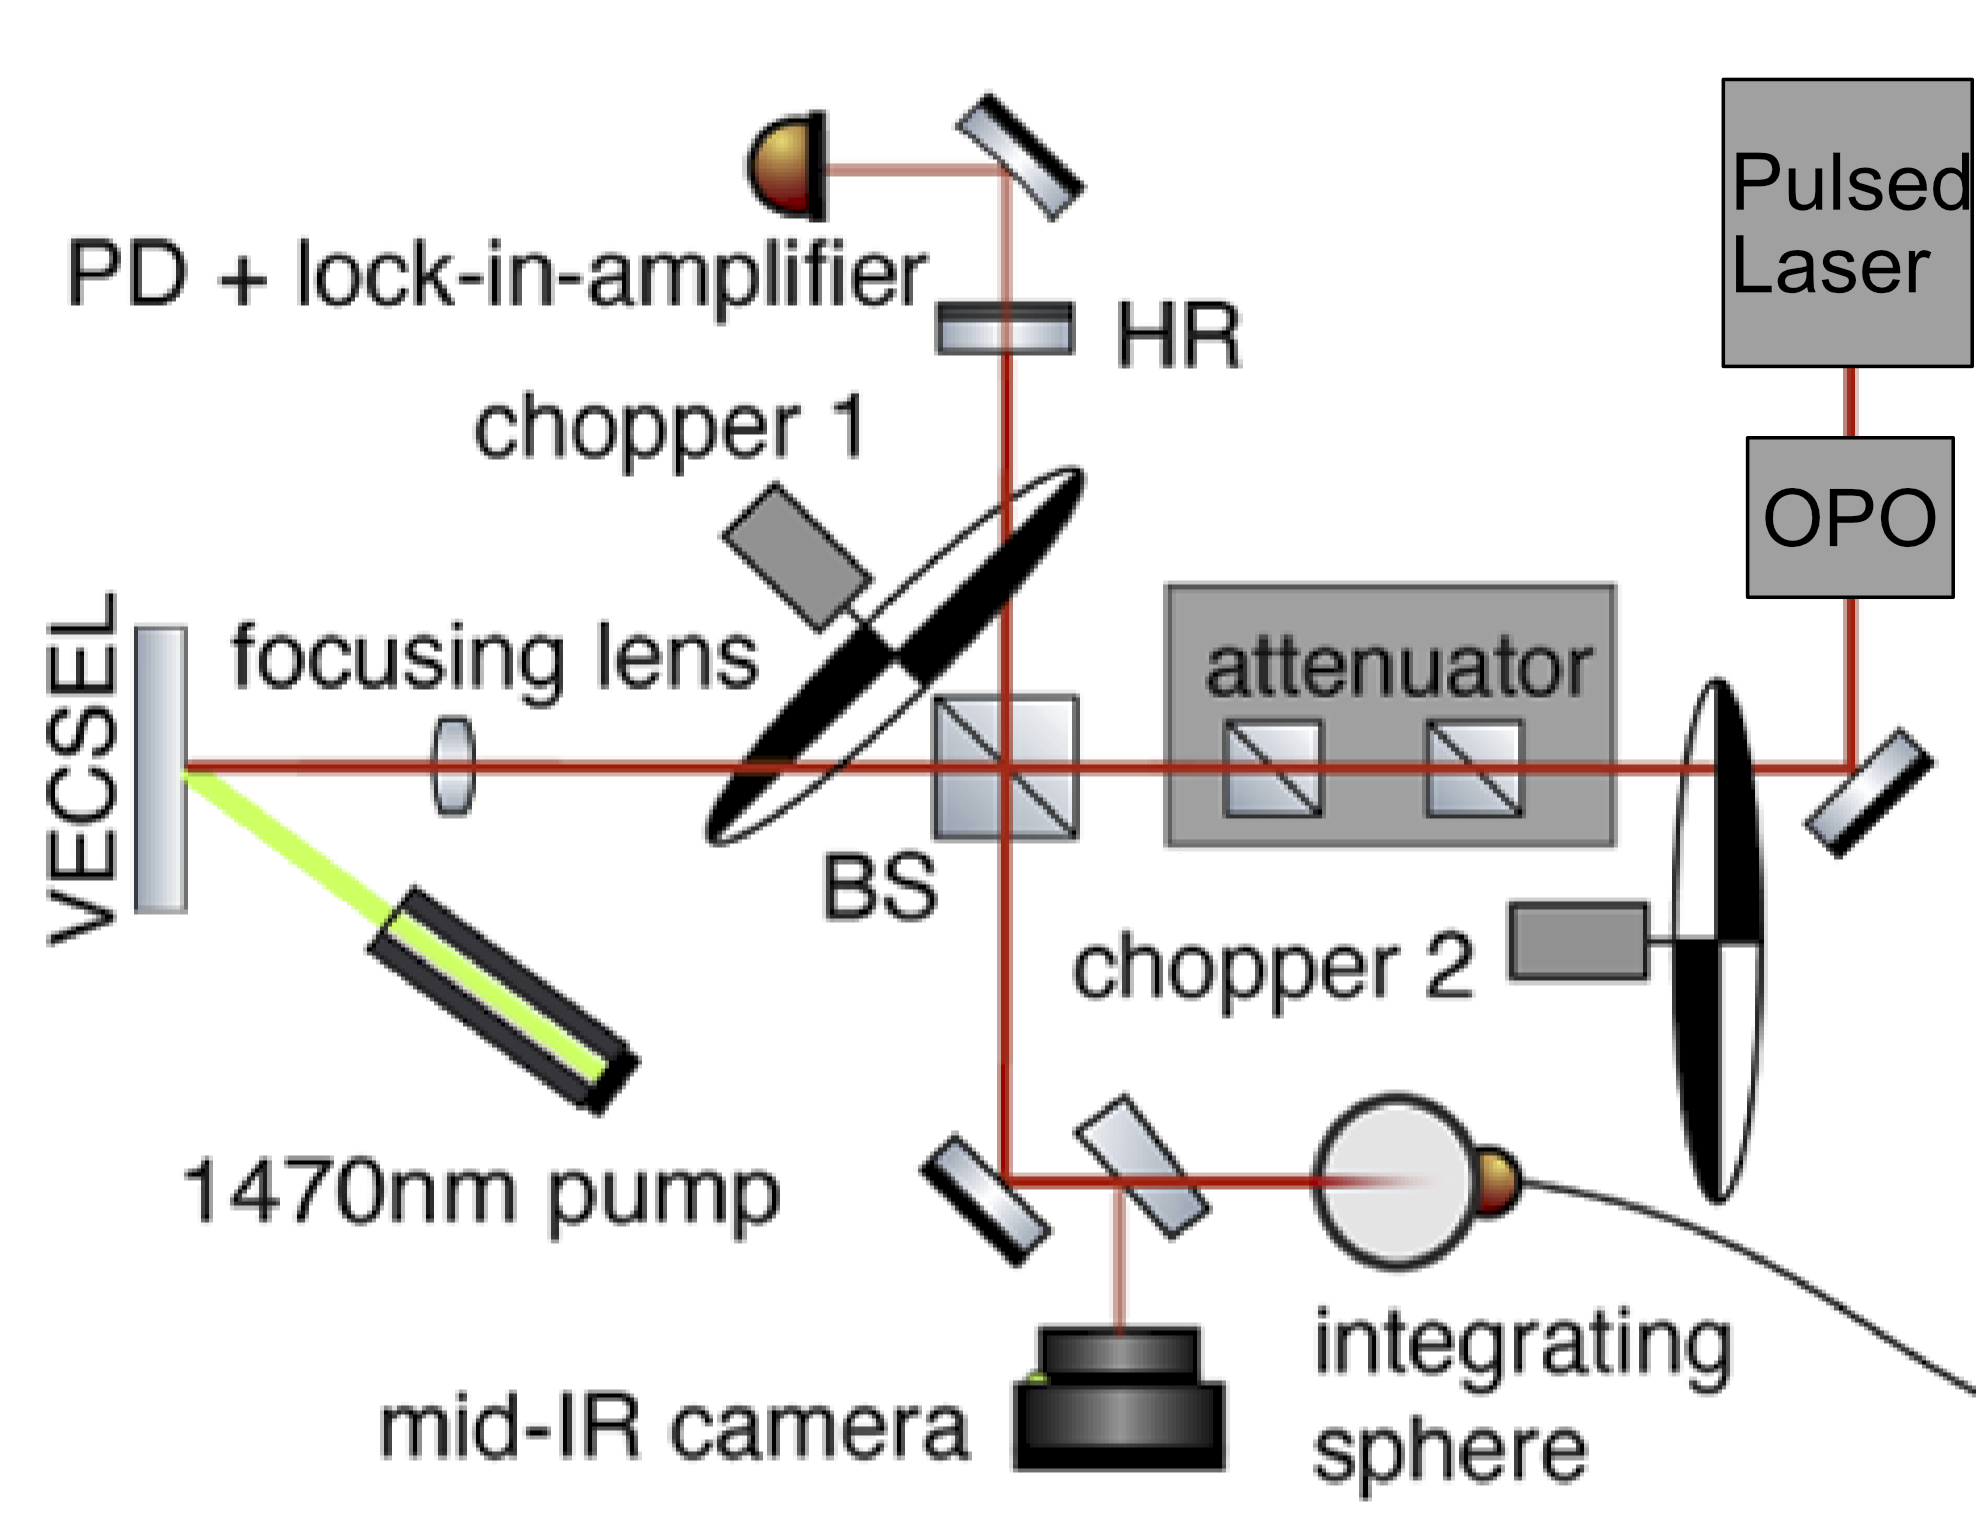
\includegraphics[width=0.8\linewidth]{images/setup.png}
    \caption{Experimental Setup for gain characterization of VECSEL chips. The laser source is a tunable optical paramtertic oscillater pumped by a modelocked Ti:sapphire laser. The beam gets attenuated. The pump beam enters the setup at a \qty{30}{\degree} angle. Two choppers, phase-locked and operating at different frequencies, are positioned to differentiate signals and measure photoluminescence (PL) emitted by the pumped VECSEL chips. The figure showcases the key components and their relative positions within the experimental setup.}
    \label{fig:setup}
\end{figure}

\subsection{Automation of the pump power}{\label{subsubsection:pump}}

In the original setup, the pump laser diode was controlled over a DC power supply, which can deliver up to \qty{50}{\ampere} at up to \qty{18}{\volt}. The power supply was operated manually in a current control mode. This required after 

Due to the choice of emasuring for 9 different pump powers for each temperatue and chip design and one measruement taking about \qty{10}{\min}. All the measuremnt would take a significant amount of time without much downtime between the measurement, since each measurement required to change the pump power and also to manually start the measuerment. Furtunately the power supply had a serial interface, which could be controlled from the software, it was only necessary to build in. This allowed to additionaly set up the current control for the pump power and measure the pump power in one go taking about \qty{90}{\min}.

\begin{figure}[ht]
    \centering
    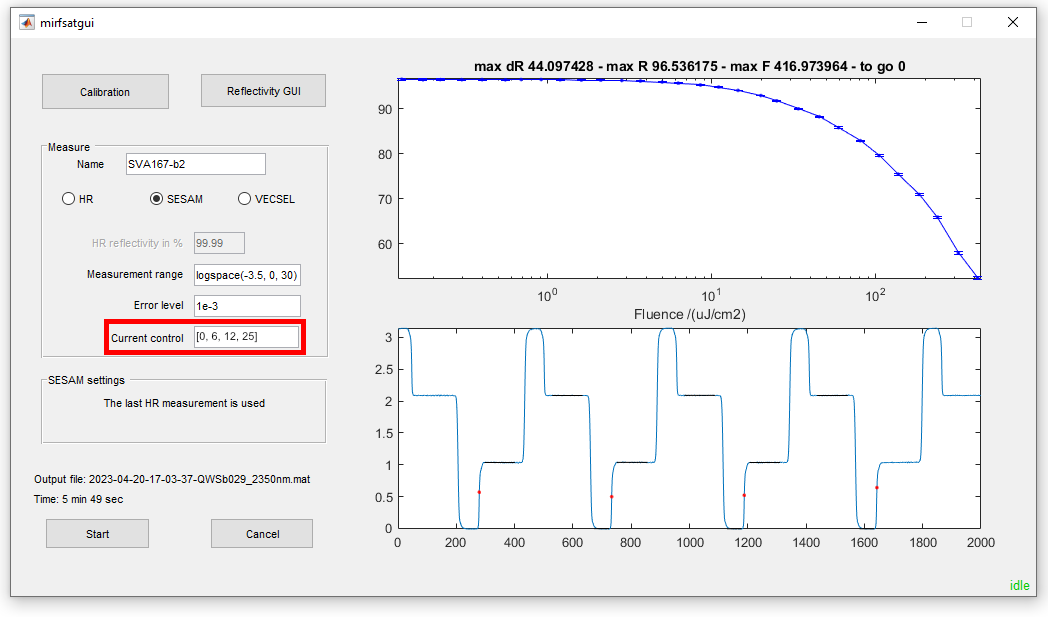
\includegraphics[width=0.8\linewidth]{images/software.png}
    \caption{}
\end{figure}
